\documentclass[../main.tex]{subfiles}
\begin{document}
\chapter{Estado del Arte}
\section{Ortoferritas de Tierras Raras}
Los óxidos de tipo perovskita (\ce{ABO3} con A una tierra rara o metal alcalinotérreo y B un metal de transición) son estructuras estudiadas muy comúnmente en el campo de la ciencia de materiales debido a sus propiedades electromagnéticas, ópticas y catalíticas, además de su estabilidad \cite{Wang2019}.

El objeto de estudio de este trabajo son las ortoferritas \ce{RFeO3}, con R una tierra rara, específicamente en los compuestos \neod{}, \sama{}, debido a que presentan un orden magnético intrínseco proveniente de su estructura cristalina. Esta misma estructura además hace posible la presencia de ferroelectricidad, lo cual daría como resultado un material multiferroico \cite{Sharma2024}.
\begin{figure}[H]
    \centering
    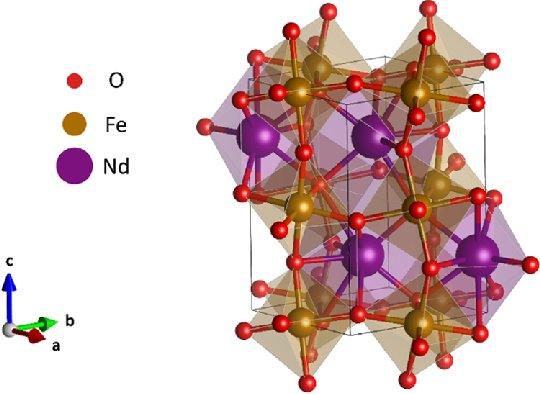
\includegraphics[width=0.5\textwidth]{fig/estructuraNd.jpg}
    \caption{Estructura cristalina del \neod{}. Tomado de \cite{Quionero2021}}
    \label{fig:estructNd}
\end{figure}

\section{Electromagnetismo en Sólidos}
La respuesta de un sólido al aplicar un campo externo, sea éste magnético o eléctrico, depende de las propiedades intrínsecas de la estructura cristalina de éste. A pesar de esto, las interacciones a nivel cuántico se manifiestan macroscópicamente como propiedades extensivas, las cuales pueden estudiarse mediante la electrodinámica clásica.

Las ecuaciones de Maxwell pueden modificarse para incluir las contribuciones dependientes de las propiedades del material, considerando que las cargas y corrientes dentro de un éste pueden moverse libremente, o estar ligadas.

Así, se puede escribir:
\begin{equation}
    \begin{split}
        \vec{E}=\varepsilon_0\vec{D}-\vec{P}\\
        \vec{B}=\mu_0(\vec{H}-\vec{M})
    \end{split}  
    \label{eq:maxwellmacro}
\end{equation}
Donde la fuente de los campos $\vec{D}$ y $\vec{H}$ son las cargas (o corrientes) libres, determinadas por la configuración del sistema, mientras que para los campos $\vec{P}$ y $\vec{M}$ son las cargas (o corrientes) ligadas, determinadas por las propiedades del material \cite{griffiths2023introduction}.
\subsection{Magnetización y Polarización en Sólidos}
Ambas propiedades representan la respuesta de la estructura a los campos externos. Macroscópicamente, pueden escribirse de la siguiente manera:
\begin{equation}
    \begin{split}
        P_{i}=\varepsilon_0\chi_{ij}^{(e)}E_j\\
        M_{i}=\chi_{ij}^{(m)}B_j
    \end{split}
    \label{eq:tensorMP}
\end{equation}
En esta expresión, $\chi_{ij}$, la susceptibilidad, representa los componentes de un tensor de $3\times3$ \cite{Damjanovic2006}.

Sin embargo, para un material isótropo, esta relación se simplifica a una multiplicación por un escalar, el cual aún puede depender de factores como la temperatura o el tiempo.
\begin{equation}
    \begin{split}
        \vec{P}=\varepsilon_0\chi^{(e)}\vec{E}\\
        \vec{M}=\chi^{(m)}\vec{B}
    \end{split}
    \label{eq:escalarMP}
\end{equation}
Por otro lado, también es posible entenderlas como la suma de una propiedad microscópica, es decir, para un volumen de material $V$ pueden escribirse como:
\begin{equation}
    \begin{split}
        \vec{P}=\sum_i \dfrac{\vec{d_i}}{V}\\
        \vec{M}=\sum_i \dfrac{\vec{m_i}}{V}
    \end{split}
    \label{eq:relacionmicromacro}
\end{equation}
Donde $\vec{m_i}$ es el momento magnético de cada electrón en el material, y $\vec{d_i}$ es el momento dipolar de cada celda unitaria \cite{Visintin2006}.
\subsection{Histéresis} \label{sec:hist}
Un fenómeno presenta histéresis si depende no sólo de las condiciones actuales del sistema, sino que también de las condiciones anteriores. Ésto ocurre para propiedades como la elasticidad, la fricción, la superconductividad, la adsorción, la desorción y, siendo éstas el objeto de estudio de este trabajo, la magnetización y la polarización.

En general, la histéresis, observada en propiedades extensivas, proviene de las contribuciones microscópicas de propiedades intensivas \cite{Visintin2006}.

Este fenómeno es evidente al aplicar un campo externo, sea este magnético o eléctrico, los dominios en el material cuya propiedad intensiva relevante sea paralela al campo aplicado serán energéticamente favorables y por lo tanto crecerán a costa de aquellos dominios orientados de forma distinta, lo que aumenta la propiedad extensiva relevante hasta alcanzar un valor máximo, conocido como campo de saturación.

Este proceso no es reversible, si se quita el campo externo el sistema no regresará por si solo a la configuración inicial, sino que tendrá una polarización, o magnetización, remanente distinta de 0. Si se busca que ésta se anule, se debe de aplicar un campo externo en sentido opuesto, conocido como campo coercitivo.
\subsection{Clasificación de Materiales}
Es posible clasificar los materiales según su respuesta a los campos externos aplicados.

Hasta ahora ambos campos han tenido relaciones análogas, sin embargo, el hecho de que sólo el campo eléctrico posea cargas, hace que existan comportamientos de la polarización que no se observan para la magnetización. Por esta razón, se discutirán por separado.
\subsubsection{Clasificación de Materiales Magnéticos}

Pueden dividirse en dos grupos, aquellos cuyo comportamiento depende únicamente de las propiedades de los electrones en la red, y aquellos que dependen de un orden intrínseco en la red. El primer grupo se compone de los siguientes materiales:
\begin{itemize}
    \item \textbf{Diamagnéticos:} Para un electrón sujeto a una órbita al cual se le aplica un campo magnético externo, la torca que éste ejerce sobre el momento magnético del electrón provoca un efecto conocido como la Precesión de Larmor, el cual consiste en una rotación periódica en el momento magnético. Ésto puede verse como una corriente que, debido a la Ley de Lens, provocará un campo magnético que se opone al campo que la generó, es decir, $\chi<0$ \cite{coey2010magnetism}.
    \item \textbf{Paramagnetismo:} Cuando un material que posee un electrón desapareado en su capa de valencia es expuesto a un campo magnético externo, favorecerá el alineamiento de los momentos magnéticos de cada electrón en el mismo eje. En particular, para los electrones desapareados, el campo favorecerá a la población paralela sobre la antiparalela, provocando una magnetización en el mismo sentido que el campo externo, es decir, $\chi>0$, siendo $\chi$ constante a campos pequeños, pero llegando a una saturación cuando todos los momentos se han alineado. Sin embargo, al retirar el campo externo, estos momentos magnéticos volverán a orientarse de forma aleatoria, regresando la magnetización a 0 \cite{coey2010magnetism}.
\end{itemize}
Por otro lado, en el segundo grupo se pueden identificar tres tipos de material:
\begin{itemize}
    \item \textbf{Ferromagnéticos:} Debido a las propiedades de su estructura cristalina, estos materiales están divididos en zonas en las que el momento magnético tiene una dirección preferencial, llamados dominios magnéticos, los cuales se vuelven energéticamente más favorables al aplicar un campo magnético paralelo en el material, por lo que comienzan a crecer a costa de las zonas en direcciones distintas, es decir, presentan histéresis. Son similares a los materiales paramagnéticos debido a que ambos provienen de una reorientación de espines, ambos tienen una $\chi>0$, y ambos poseen un campo de saturación $M_s$, sin embargo, como se discutió en la sección \ref{sec:hist}, al presentar histéresis estos también poseen magnetización remanente $M_r$, la cual se cancela con un campo coercitivo $H_c$ \cite{coey2010magnetism}.
    \item \textbf{Antiferromagnéticos:} De manera similar a los materiales ferromagnéticos, estos también presentan dominios magnéticos, y por tanto histéresis, sin embargo, estos dominios poseen no solo electrones apuntando con un momento magnético en una dirección, sino también electrones cuyo momento magnético apunta en dirección opuesta, ambos de igual magnitud, por lo que $M=0$ \cite{coey2010magnetism}.
    \item \textbf{Ferrimagnéticos:} Finalmente, los materiales ferrimagnéticos son similares a los antiferromagnéticos, también poseen dominios con electrones cuyos momentos magnéticos apuntan en direcciones opuestas, sin embargo los momentos en una dirección son más pequeños que los momentos en la otra, lo cual provoca una magnetización positiva, aunque menor a la de los materiales ferrimagnéticos \cite{coey2010magnetism}.
\end{itemize}
\subsubsection{Clasificación de Materiales Eléctricos}
\subsection{Multiferroicidad}
\end{document}